\documentclass[xcolor=dvipsnames]{beamer}
\usecolortheme[named=PineGreen]{structure} 
\useoutertheme{infolines} 
\usetheme[height=7mm]{Rochester} 
\usefonttheme{structuresmallcapsserif}
\setbeamertemplate{items}[ball] 
\setbeamertemplate{blocks}[rounded][shadow=true] 
\setbeamertemplate{navigation symbols}{} 
\usepackage{tikz}
\usepackage{ellipsis}

\author{Wim Looman}
\title{Software Engineering}
\subtitle{In the Mariokart system}
\institute[UC]
{
  Department of Electrical Engineering\\
  University of Canterbury\\
  New Zealand
}
\date{26 September, 2011}

\begin{document}
  \begin{frame}[plain]
    \titlepage
  \end{frame}

  \begin{frame}{Outline}
    \begin{center}
      \begin{minipage}{0.5\linewidth}
        \tableofcontents
      \end{minipage}
    \end{center}
  \end{frame}

  \section{Continuous Integration}
    \subsection{What is it?}
      \begin{frame}{What Is Continuous Integration?}
        \begin{center}\begin{minipage}{0.8\linewidth}\begin{block}{Definition\footnotemark}

              \emph{``Continuous Integration is a software development
              practice~\dots\ leading to multiple integrations per day~\dots\
              verified by an automated build~\dots\ to detect integration errors
              as quickly as possible.''}~---~Martin Fowler

        \end{block}\end{minipage}\end{center}

        \footnotetext{\url{http://martinfowler.com/articles/continuousIntegration.html}}
      \end{frame}

    \subsection{Why would you use it?}
      \begin{frame}{Why Would You Use Continuous Integration?}
        \Large
        \begin{itemize}
          \pause\item Detect errors early.
          \vspace{\baselineskip}
          \pause\item Minimizes time between error introduction and fix.
          \vspace{\baselineskip}
          \pause\item Provides a stable base for future work.
          \begin{itemize}
            \pause \item \large Very useful for branch-happy development in git.
          \end{itemize}
          \vspace{\baselineskip}
          \pause\item Peer pressure
                
\includegraphics[height=11pt]{images/smiley-devil}.
        \end{itemize}
      \end{frame}

    \subsection{CI Joe}
      \begin{frame}{CI Joe\footnotemark}
        \only<1>{
          \begin{center}\begin{minipage}{0.65\linewidth}\begin{block}{Repository Description}
            \emph{``CI Joe is a fun Continuous Integration server.''}
          \end{block}\end{minipage}\end{center}
        }

        \only<2->{
          \begin{itemize}
            \Large
            \item<2-> Simple setup.
            \vspace{\baselineskip}
            \item<3-> Designed to work with git.
            \vspace{\baselineskip}
            \item<4-> Can trigger a build via a post-hook on github.
            \vspace{\baselineskip}
            \item<5-> Reports status via build-hook (used to send email).
          \end{itemize}
        }

        \footnotetext[2]{\url{https://github.com/defunkt/cijoe}}
      \end{frame}

    \subsection{Did it help?}
      \begin{frame}{Did Continuous Integration Help?}
      \end{frame}

    \subsection{Examples}
      \begin{frame}{Example 1}
        \only<1>{
          %
\includegraphics[width=0.45\linewidth]{images/green-dashboard}
          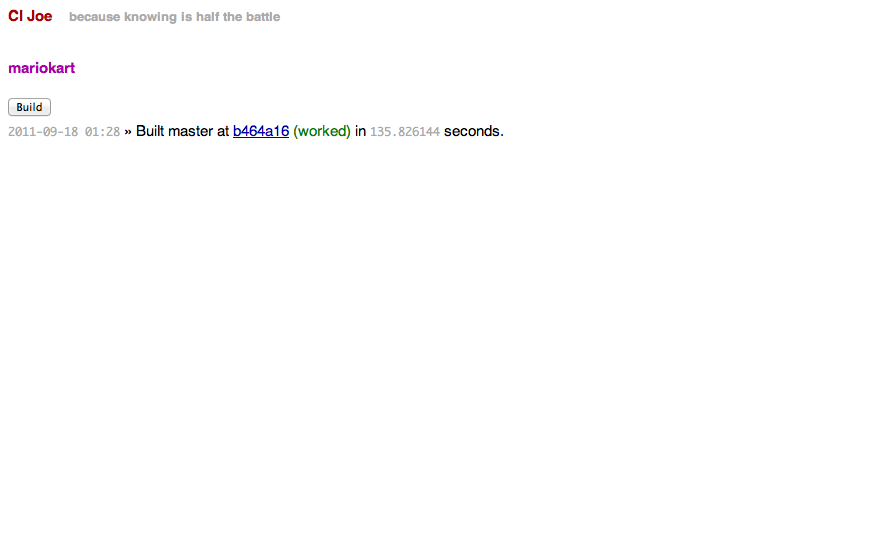
\includegraphics[width=\linewidth]{images/green-full}
        }
        \only<2>{
          %
\includegraphics[width=0.45\linewidth]{images/building-dashboard}
          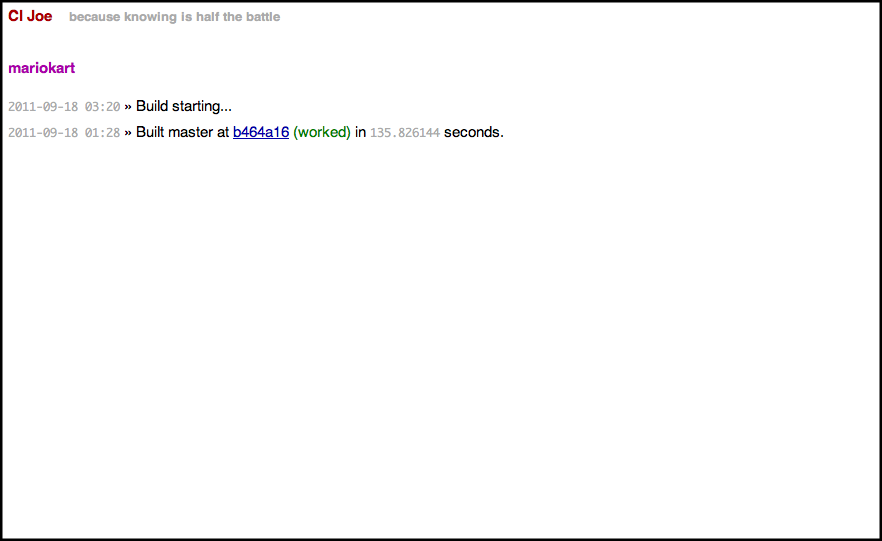
\includegraphics[width=\linewidth]{images/building-full}
        }
        \only<3>{
          %
\includegraphics[width=0.45\linewidth]{images/fail-dashboard}
          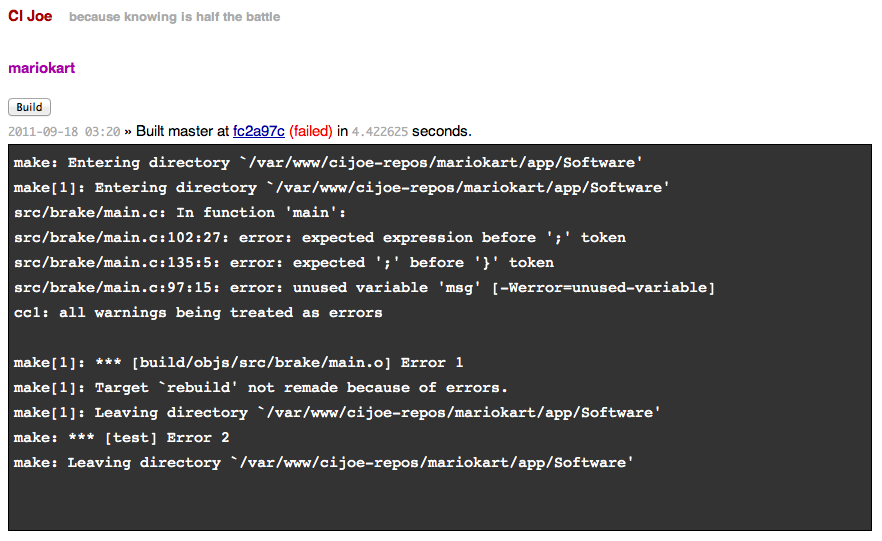
\includegraphics[width=\linewidth]{images/fail-full}
        }
      \end{frame}

      \begin{frame}{Example 2}
        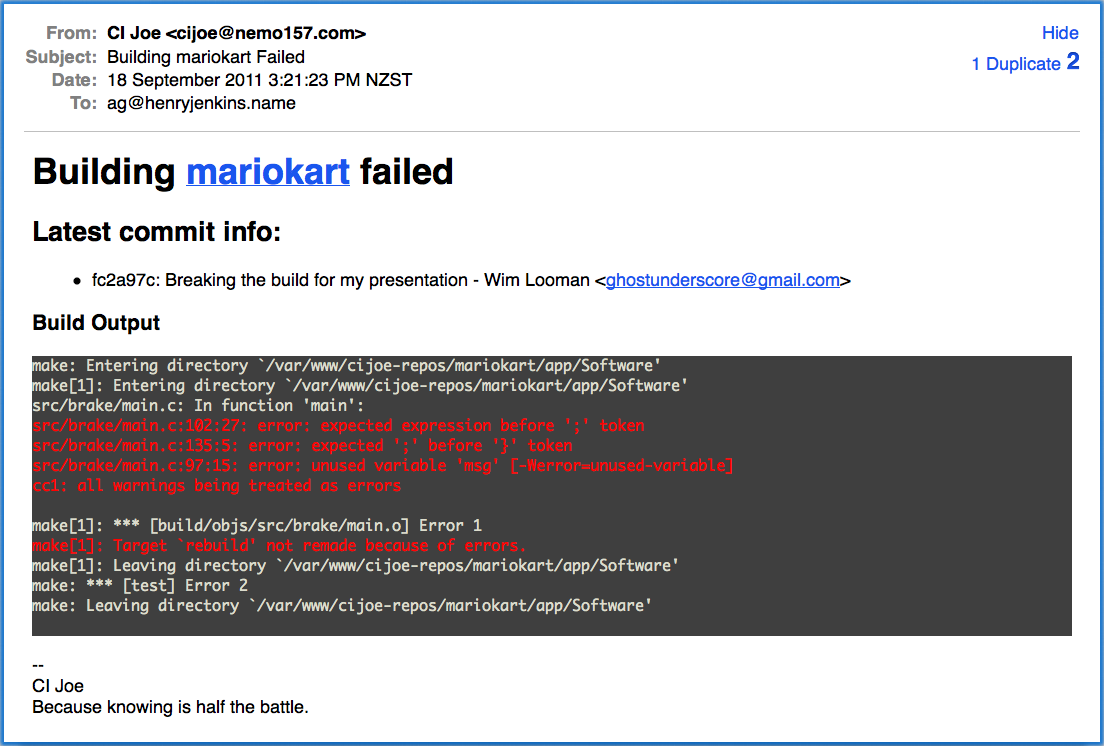
\includegraphics[width=\linewidth]{images/email}
      \end{frame}

    \section{Questions}
      \begin{frame}[plain]
        \begin{tikzpicture}[remember picture,overlay]
          \node[at=(current page.center)] {
            
\includegraphics[width=\paperwidth]{images/mario_kart_lego}
          };
        \end{tikzpicture}
      \end{frame}
\end{document}
